\begin{figure}[t]
	\centering

	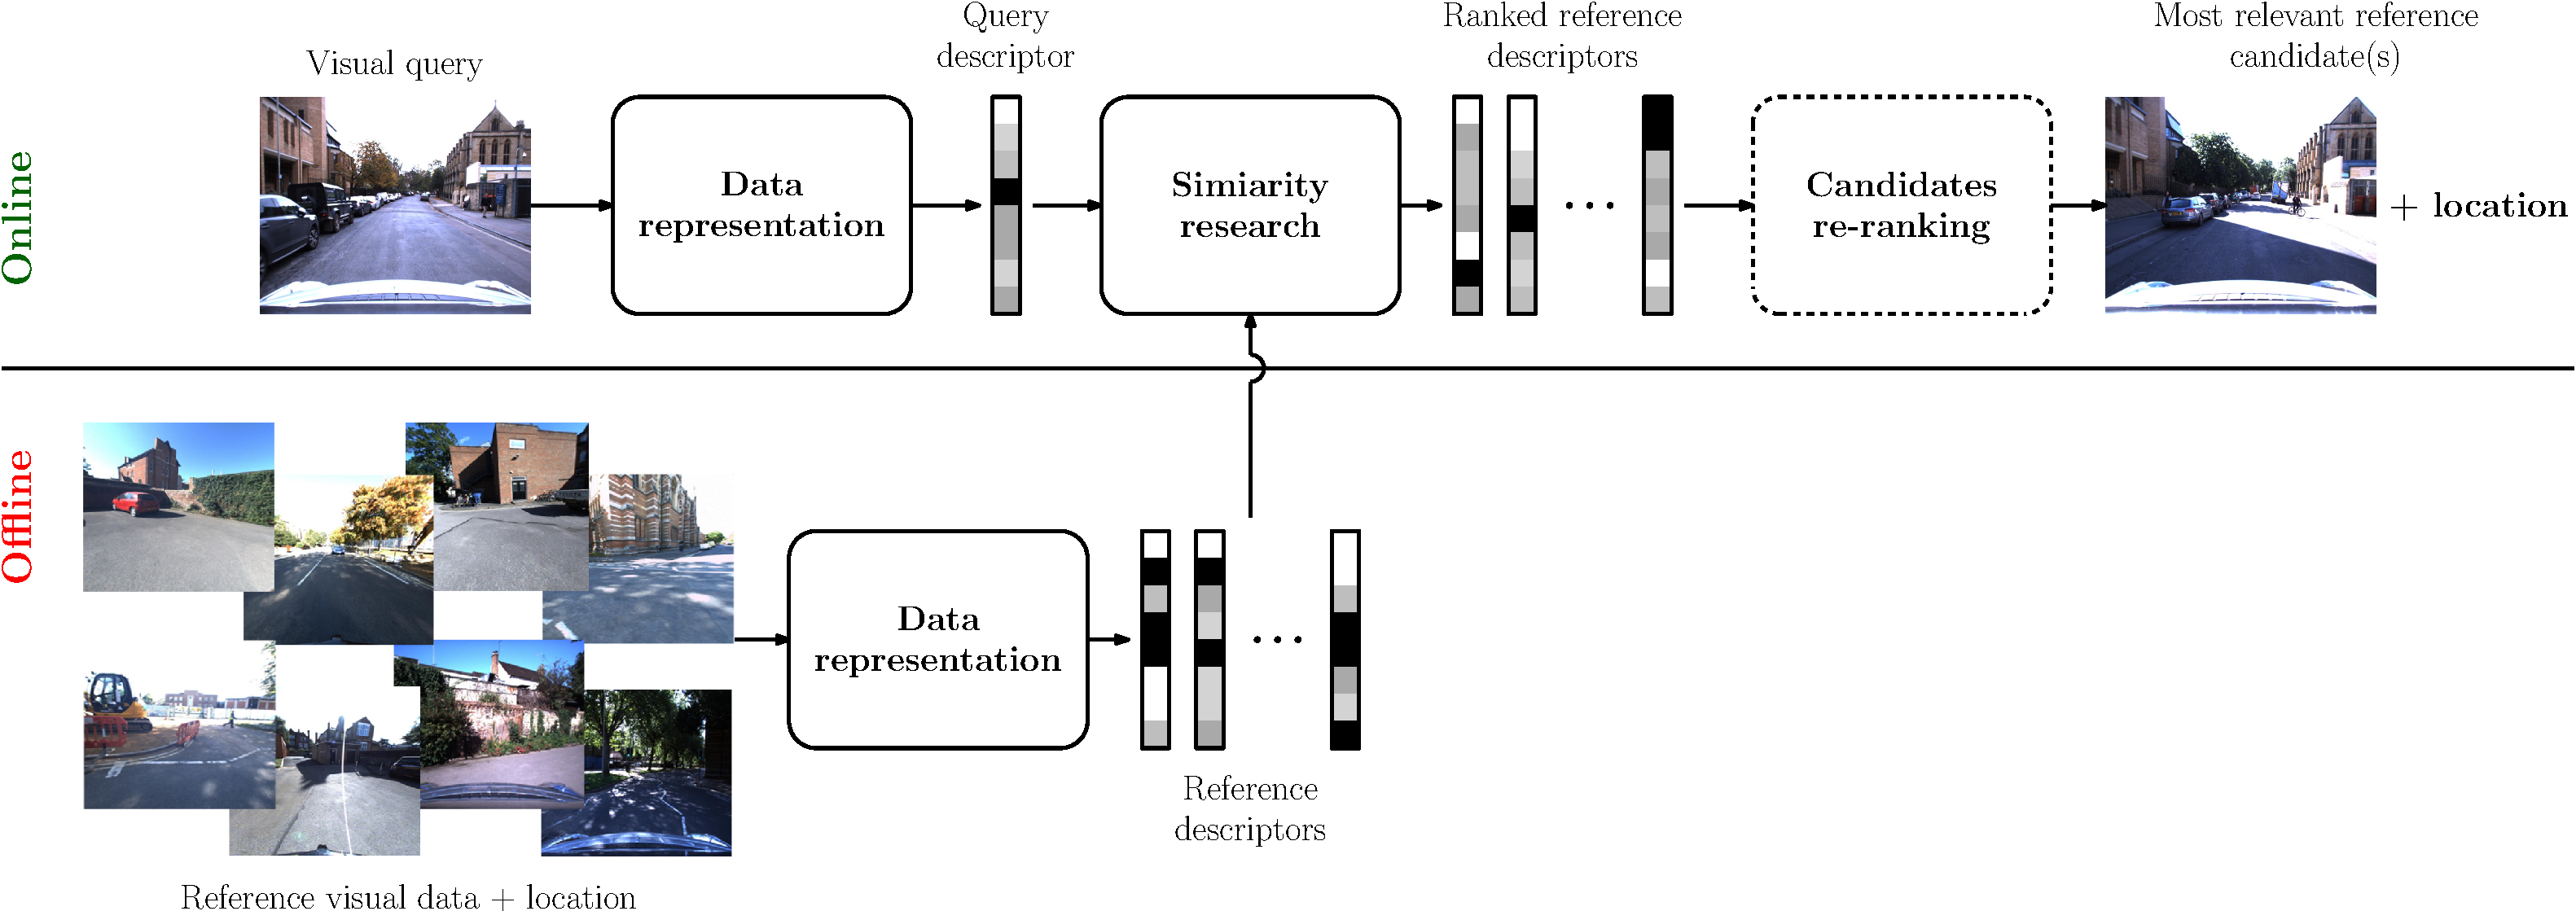
\includegraphics[width=\linewidth]{methods/cbir_for_localization}
	\caption[CBIR for localization]{\label{fig:cbir_for_localization}\textbf{CBIR for localization:} the location of a given request can be retrieved by comparing the query to a pool of geolocalized candidates. After the similarity comparison, the location associated to the top-ranked reference data is considered as the location of the query. Re-ranking of the reference data can be used in order to improve the relevance of the top-ranked candidates.}
\end{figure}
